\section{Podstawy obsługi systemu operacyjnego QNX RTOS}

\subsection{Powłoka}

Powłoka:

\begin{myitemize}
\item Interpreter poleceń użytkownika
\item Pośredniczy między użytkownikiem a systemem
\item Środowisko pracy użytkownika w systemie
\item Przetwarza pojedyncze polecenie lub skrypty
\end{myitemize}


\begin{example}[Przykład prostej komendy] \label{ex:prostakomenda}

Polecenia można wydawać powłoce z wiersza poleceń (terminala, konsoli) wpisując ich nazwy.

\begin{lstlisting}[style=MyBashStyle]
# ls
\end{lstlisting}

Komenda wyświetla zawartość bieżącego katalogu.
\end{example}

\begin{example}[Przykład komendy z~argumentami]\label{ex:prostakomenda2}
%\addcontentsline{toc}{subsubsection}{Przykład \ref{ex:prostakomenda2}}

Komenda wyświetla zawartość bieżącego katalogu wraz ze szczegółowymi informacjami nt. obiektów. Argumenty (\lstinline[style=MyBashStyle]{-l}) zmieniają zachowanie komendy prostej.

\begin{lstlisting}[style=MyBashStyle]
# ls -l
\end{lstlisting}


Formalna składnia komendy z argumentami:

\begin{lstlisting}[style=MyBashStyle]
# command argument1 argument2 argument3 ... argumentN
\end{lstlisting}
\end{example}

\begin{example}[Przykład złożonej komendy]\label{ex:prostakomenda3}

Komendy proste i~komendy proste z~argumentami możemy łączyć. Separatorem poleceń jest średnik (\lstinline[style=MyBashStyle]{;}).


\begin{lstlisting}[style=MyBashStyle]
# date ; ls
\end{lstlisting}

Formalna składnia złożonej komendy:

\begin{lstlisting}[style=MyBashStyle]
# command1; command2; command3; ... argumentN
\end{lstlisting}
\end{example}

\begin{example}[Logowanie do systemu z wiersza poleceń]\label{ex:prostakomenda4}


Aby zalogować się do systemu z wiersza poleceń używamy polecenia \lstinline[style=MyBashStyle]{login}.

\begin{lstlisting}[style=MyBashStyle]
# login
# login: root
\end{lstlisting}

Polecenie uzyskuje od użytkownika jego nazwę oraz hasło, które następnie weryfikuje z danymi zawartymi w pliku \lstinline[style=MyBashStyle]{/etc/passwd}, który możemy podejrzeć poleceniem \lstinline[style=MyBashStyle]{cat}.
\end{example}


\begin{example}[Plik definiujący użytkowników systemu]\label{ex:prostakomenda5}


Po zalogowaniu przez polecenie \lstinline[style=MyBashStyle]{login} wywoływana jest powłoka (\lstinline[style=MyBashStyle]{/bin/sh}). Następnie w fazie inicjalizacji, ustawiane są parametry pracy powłoki. Na ogół jest to proces dwuetapowy, w~którym interpretowane są pliki \lstinline[style=MyBashStyle]{/etc/passwd} oraz \lstinline[style=MyBashStyle]{.profile} z domowego katalogu. Obejrzeć zawrtość pliku \lstinline[style=MyBashStyle]{/etc/passwd}.

\begin{lstlisting}[style=MyBashStyle]
# cat /etc/passwd
\end{lstlisting}
\end{example}

\begin{example}[Wejście i wyjście z powłoki]\label{ex:prostakomenda6}


Powłoka wykonuje polecenia użytkownika. Kiedy powłoka wyświetla znak zachęty, który w domyślnym shell-u (Bourne shell) w systemie QNX jest znak \lstinline[style=MyBashStyle]{#} dla użytkownika \lstinline[style=MyBashStyle]{root}, to czeka na polecenia użytkownika. Możemy uruchomić powłokę w takim trybie. Sytuację tę ilustruje poniższy przykład.


\begin{lstlisting}[style=MyBashStyle]
# /bin/sh
#
# exit
\end{lstlisting}

Aby wyjść z powłoki należy użyć polecenia \lstinline[style=MyBashStyle]{# exit}.
\end{example}

\begin{example}[Obsługa edytora tekstu vi]\label{ex:vi}


Edytor \lstinline[style=MyBashStyle]{vi} jest zaawansowanym edytorem tekstowym często występującym w~systemach Unix. Aby uruchomić edytor należy wpisać komendę:

\begin{lstlisting}[style=MyBashStyle]
# vi
\end{lstlisting}

 Edytor \lstinline[style=MyBashStyle]{vi} jest edytorem modalnym. Oznacza to, że może znajdować się w~dwóch stanach: \textbf{trybie edycji} lub \textbf{trybie poleceń}.

\begin{itemize}
\item Przejście do trybu edycji poprzez wydanie polecenia \lstinline[style=MyBashStyle]{i} (insert) lub \lstinline[style=MyBashStyle]{a} (append).
\item Przejcie z~trybu edycji do trybu poleceń odbywa się poprzez naciśnięcie klawicza \lstinline[style=MyBashStyle]{Esc}.
\end{itemize}

Polecenia edytora \lstinline[style=MyBashStyle]{vi} składają się z~kilku grup. Przedstawiono je zbiorczo w~postaci krótkiej instrukcji na stronie~\pageref{viRef}.
\end{example}

\clearpage
\phantomsection
{\label{viRef}
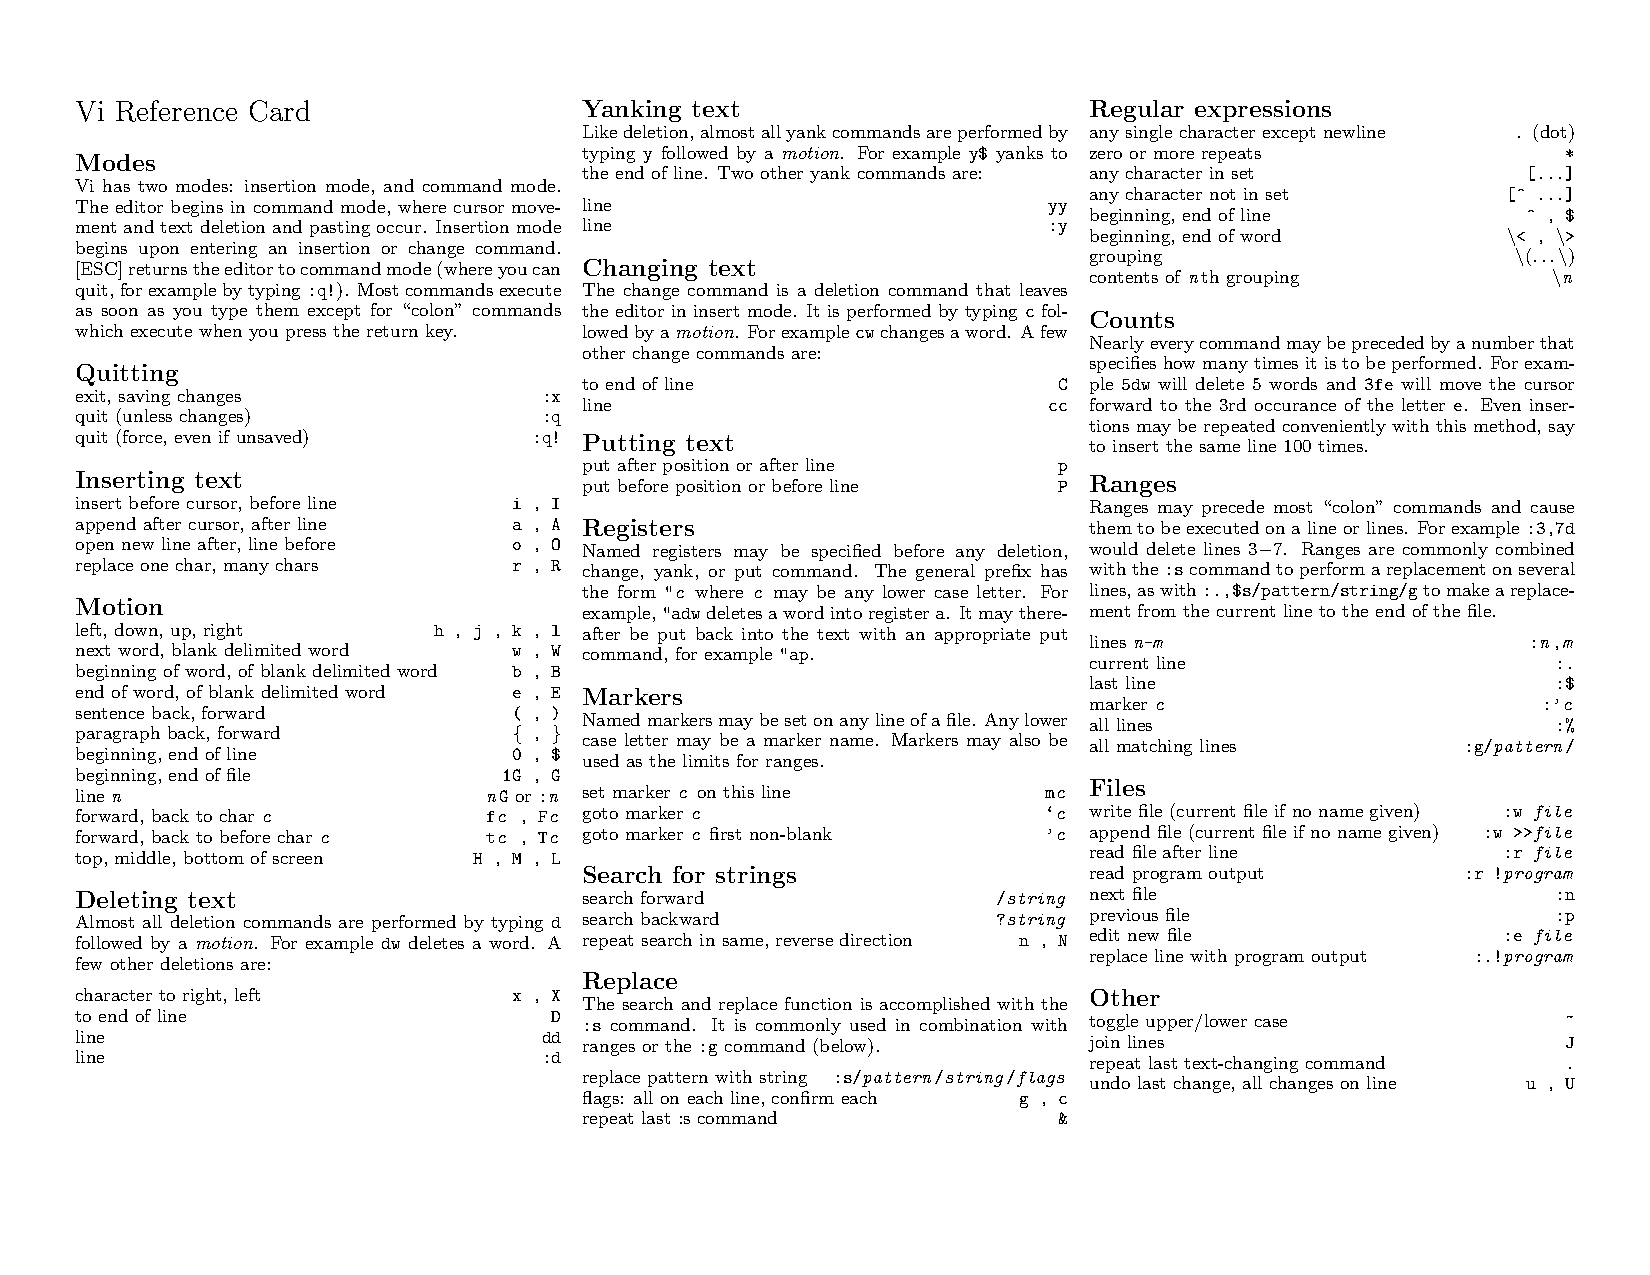
\includepdf[scale=0.95,pages={1},pagecommand={\thispagestyle{fancy}},pagecommand={\thispagestyle{fancy}{\label{subsec:vi}}},lastpage=1,angle=90]{img/viRef.pdf}
}



\begin{example}[Utworzenie i~uruchomienie skryptu] \label{ex:prostakomenda7}


Powłoka, jako interpreter, wykonuje pewien program.  Kolejne komendy programu mogą być wpisywane na bieżąco w~terminalu lub cały program może być dostarczony do powłoki w~postaci skryptu. Należy utworzyć plik o~nazwie \lstinline[style=MyBashStyle]{skrypt} edytorem tekstu \lstinline[style=MyBashStyle]{vi} o~treści:

\begin{lstlisting}[style=MyBashStyle]
date ; ls
\end{lstlisting}

W~następnej kolejności uruchomić skrypt powłoki wydając polecenie:

\begin{lstlisting}[style=MyBashStyle]
# /bin/sh skrypt
\end{lstlisting}

Przykład ilustruje skrypt powłoki. Na ogół skrypty składają się z plików, w których są zapisane komendy, interpretowane przez powłokę. Skrypt można uruchomić wpisując w wiersz poleceń jego nazwę. Jednak bezpośrednie wpisanie jego nazwy kończy się niepowodzeniem:

\begin{lstlisting}[style=MyBashStyle]
# ./skrypt
sh: ./skrypt: cannot execute - Permission denied
\end{lstlisting}

W tej sytuacji należy zapewnić, aby skrypt miał odpowiednie atrybuty oraz upewnić się, że uruchamiany jest właściwy interpreter poleceń. Aby zmienić atrybuty pliku należy użyć następującego polecenia:

\begin{lstlisting}[style=MyBashStyle]
# chmod a+x ./skrypt
\end{lstlisting}

Uruchomić \lstinline[style=MyBashStyle]{skrypt} w~linii poleceń.
\end{example}


\begin{example}[Prosty skrypt powłoki]\label{ex:prostakomenda8}


Należy także uzupełnić plik \lstinline[style=MyBashStyle]{skrypt}, tak, żeby miał postać:

\begin{lstlisting}[style=MyBashStyle]
#!/bin/sh
# wypisz date i wyswietl zawartosc katalogu
date ; ls
\end{lstlisting}

Znak \lstinline[style=MyBashStyle]{#} stanowi znak komentarza w~skrypcie. Wiersze zaczynające się od tego znaku są ignorowane przez interpreter poleceń i~traktowane jako komentarz, oprócz pierwszej linii z~komendą \lstinline[style=MyBashStyle]{#!/bin/sh}. Pierwsza linia kodu przekazuje informacje o~rodzaju powłoki, która powinna wykonać skrypt.
\end{example}


\begin{example}[Prosty skrypt powłoki]\label{ex:prostakomenda9}

Dokumentacja systemu jest dostępna w formie elektronicznej na stronach \href{www.qnx.com}{www.qnx.com}. Skrócony opis interesującego nas polecenia systemowego uzyskujemy poprzez wpisanie w okno terminala polecenia \lstinline[style=MyBashStyle]{use polecenie}, np.:

\begin{lstlisting}[style=MyBashStyle]
# use date
\end{lstlisting}
\end{example}

\subsection{System plików}

W systemie QNX Neutrino prawie wszystkie zasoby są plikami. Dane, urządzenia, bloki pamięci, a nawet pewne usługi są reprezentowane przez abstrakcję plików. Mechanizm plików pozwala na jednolity dostęp do zasobów zarówno lokalnych, jak i~zdalnych, za pomocą poleceń i programów usługowych wydawanych z okienka poleceń. Typowe drzewo plików w~systemie QNX przedstawiono na rysunku~\ref{fig:drzewo}.

\begin{figure}[!h]
\centering
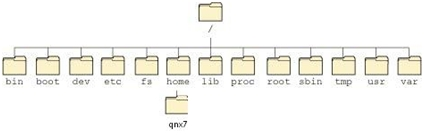
\includegraphics[width=0.75\textwidth]{img/systemplikow}
\caption{Drzewo plików w systemie QNX}
\label{fig:drzewo}
\end{figure}

\begin{myitemize}
\item Katalog główny \lstinline[style=MyBashStyle]{/} jest miejscem montowania twardego dysku lub pamięci flash.
\item \lstinline[style=MyBashStyle]{/bin} - zawiera podstawowe komendy systemowe (np. \lstinline[style=MyBashStyle]{ls}, \lstinline[style=MyBashStyle]{chmod}).
\item \lstinline[style=MyBashStyle]{/boot} - zawiera pliki i katalogi związane z obrazami systemu operacyjnego.
\item \lstinline[style=MyBashStyle]{/dev} - katalog przynależy do menadżera zasobów, w którym przechowywane są informacje o urządzeniach dostępnych w systemie.
\item \lstinline[style=MyBashStyle]{/etc} - zawiera pliki i programy używane do administracji i konfiguracji systemu.
\item \lstinline[style=MyBashStyle]{/fs} - w katalogu są montowane dodatkowe systemy plików.
\item \lstinline[style=MyBashStyle]{/home} - katalogi domowe użytkowników.
\item \lstinline[style=MyBashStyle]{/lib} - zawiera współdzielone biblioteki używane przez inne programy, procesy.
\item \lstinline[style=MyBashStyle]{/proc} - katalog, w którym są zawarte informacje o procesach i przestrzeni nazw.
\item \lstinline[style=MyBashStyle]{/root} - katalog domowy dla użytkownika root.
\item \lstinline[style=MyBashStyle]{/sbin} - zawiera niezbędne pliki wykonywalne (np. sterowniki, programy inicjujące, konfiguracyjne, menadżery).
\item \lstinline[style=MyBashStyle]{/tmp} - zawiera pliki tymczasowe.
\item \lstinline[style=MyBashStyle]{/usr} - zawiera współdzielone dane, tylko do odczytu.
\item \lstinline[style=MyBashStyle]{/var} - zawiera zmienne dane (np. cache, logi).
\end{myitemize}

W systemie QNX występują różne typy plików. Ich zestawienie przedstawiono w~tabeli \ref{tab:typyplikow}.


\begin{table}[h!]
\centering
\caption{Typy plików w~systemie QNX}
\setlength{\arrayrulewidth}{1pt}
\setlength{\tabcolsep}{6pt}
\renewcommand{\arraystretch}{1.2}
\begin{tabular}{ |p{0.15\textwidth}|p{0.3\textwidth}|p{0.4\textwidth}| }
\hline \rowcolor{gray}
\textbf{Oznaczenie} & \textbf{Typ pliku} & \textbf{Opis} \\ \hline
\mbox{\lstinline[style=MyBashStyle]{d}} & Katalog (ang. directory) & Plik zawierający inne pliki i katalogi. \\ \hline
\mbox{\lstinline[style=MyBashStyle]{l}} & Dowiązanie symboliczne (ang. symbolic link) & Dodatkowa nazwa pliku, który jest umieszczony w innym miejscu. \\ \hline
\mbox{\lstinline[style=MyBashStyle]{n}} & Plik specjalny & Np. blok pamięci współdzielonej. \\ \hline
\mbox{\lstinline[style=MyBashStyle]{c}} & Specjalny plik znakowy (ang. charakter device) & Urządzenie z dostępem znakowym (konsola, porty szeregowe, równoległe). \\ \hline
\mbox{\lstinline[style=MyBashStyle]{p}} & Plik specjalny FIFO & Bufor cykliczny w pamięci operacyjnej. \\ \hline
\mbox{\lstinline[style=MyBashStyle]{b}} & Specjalny plik blokowy (ang. block device) & Urządzenie z dostępem blokowym (dysk, partycja dyskowa). \\ \hline
\mbox{\lstinline[style=MyBashStyle]{s}} & Gniazdko (ang. socket)	 & Plik komunikacji sieciowej. \\ \hline
\end{tabular}
\label{tab:typyplikow}
\end{table}


Pliki są zorganizowane w katalogi. Katalogi mają strukturę drzewa z korzeniem \lstinline[style=MyBashStyle]{/} (\lstinline[style=MyBashStyle]{root}). Aby wskazać na konkretny obiekt w systemie plików, należy podać jego ścieżkę. Rozróżniamy ścieżki absolutne i~względne. Ścieżka absolutna zaczyna się od znaku \lstinline[style=MyBashStyle]{/} , np. \lstinline[style=MyBashStyle]{/etc/passwd}. Ścieżka relatywna zaczyna się od znaku innego niż \lstinline[style=MyBashStyle]{/} , np. \lstinline[style=MyBashStyle]{etc/passwd} .


\begin{example}[Wylistowanie zawartości katalogu]\label{ex:wylistowanie}

Pokazać zawartość bieżącego katalogu:

\begin{lstlisting}[style=MyBashStyle]
# ls -l
total 419571
drwxr-xr-x   2 root      root           3072 Feb 23  2014 bin
drwxr-xr-x   4 root      root           1024 Feb 23  2014 boot
dr-xr-xr-x   2 root      root              0 Oct 22 15:07 dev
drwxr-xr-x  10 root      root           3072 Feb 23  2014 etc
drwxr-xr-x   2 root      root           1024 Feb 23  2014 home
drwxr-xr-x   4 root      root           5120 Feb 23  2014 lib
drwxr-xr-x   3 root      root           1024 Feb 23  2014 libexec
dr-xr-xr-x   2 root      root      214798336 Oct 22 15:07 proc
drwxr-xr-x   2 root      root           1024 Sep 30 21:43 root
drwxr-xr-x   2 root      root           3072 Feb 23  2014 sbin
-rw-rw-rw-   1 root      root             11 Oct 22 12:14 skrypt
drwxr-xr-x   2 root      root           1024 Oct 22 12:30 tmp
drwxr-xr-x   7 root      root           1024 Feb 23  2014 usr
drwxr-xr-x   4 root      root           1024 Feb 23  2014 var
\end{lstlisting}

Pokazać zawartość innego katalogu:

\begin{lstlisting}[style=MyBashStyle]
# ls -la /usr/
\end{lstlisting}

Argument \lstinline[style=MyBashStyle]{-l} służy do listowania w formacie tzw. długim, natomiast argument \lstinline[style=MyBashStyle]{-a} do listowania ukrytych plików. Sprawdzić inne parametry polecenia ls następująco:

\begin{lstlisting}[style=MyBashStyle]
# use ls
\end{lstlisting}
\end{example}

\begin{example}[Obejrzenie zawartości pliku]\label{ex:obejrzenie}

Oprócz listowania zawartości katalogów, istotna jest możliwość oglądania zawartości plików (np. skryptowych):

\begin{lstlisting}[style=MyBashStyle]
# cat /skrypt
# cat -n /skrypt			# -n numerowanie linii
# cat -n /etc/passwd
\end{lstlisting}
\end{example}


\begin{example}[Wyświetlanie liczby wierszy, słów i~bajtów zawartych w pliku]\label{ex:wys}

Aby uzyskać informację o całkowitej liczbie linii, słów i~znaków, zawartych w pliku można użyć polecenie \lstinline[style=MyBashStyle]{wc} (ang. word count):

\begin{lstlisting}[style=MyBashStyle]
# wc /skrypt
\end{lstlisting}

Dostępne argumenty polecenia przedstawiono w~tabeli \ref{tab:opcjeWC}.


\begin{table}[h!]
\centering
\caption{Opcje polecenia wc}
\setlength{\arrayrulewidth}{1pt}
\setlength{\tabcolsep}{6pt}
\renewcommand{\arraystretch}{1.2}
\begin{tabular}{ |p{0.15\textwidth}|p{0.4\textwidth}|}
\hline \rowcolor{gray}
\textbf{Argumenty} & \textbf{Opis} \\ \hline
\mbox{\lstinline[style=MyBashStyle]{-l}} & Oblicza liczbę linii \\ \hline
\mbox{\lstinline[style=MyBashStyle]{-w}} & Oblicza liczbę słów \\ \hline
\mbox{\lstinline[style=MyBashStyle]{-m}} & Oblicza liczbę znaków \\ \hline
\mbox{\lstinline[style=MyBashStyle]{-c}} & Oblicza liczbę znaków  \\ \hline
\end{tabular}
\label{tab:opcjeWC}
\end{table}

\begin{example}[Poruszanie się po systemie plików]

System operacyjny jest wyposażony w zestaw instrukcji, które umożliwiają poruszanie się po drzewie plików. Najważniejsze zestawiono w tabeli~\ref{tab:poruszanie} i~zilustrowano w przykładzie.

\begin{table}[h!]
\centering
\caption{Poruszanie się po systemie plików}
\setlength{\arrayrulewidth}{1pt}
\setlength{\tabcolsep}{6pt}
\renewcommand{\arraystretch}{1.2}
\begin{tabular}{ |p{0.15\textwidth}|p{0.4\textwidth}|}
\hline \rowcolor{gray}
\textbf{Polecenie} & \textbf{Opis} \\ \hline
\mbox{\lstinline[style=MyBashStyle]{pwd}} & Wyświetlenie nazwy katalogu bieżącego (ang. print working directory) \\ \hline
\mbox{\lstinline[style=MyBashStyle]{cd}}  & Zmiana katalogu bieżącego (ang. change directory) \\ \hline
\mbox{\lstinline[style=MyBashStyle]{cd..}} & Przejście do katalogu nadrzędnego \\ \hline
\mbox{\lstinline[style=MyBashStyle]{cd /}} & Przejście do katalogu głównego \\ \hline
%\mbox{\lstinline[style=MyBashStyle]{cd ~}} &	Przejście do katalogu domowego \\ \hline
\end{tabular}
\label{tab:poruszanie}
\end{table}
\end{example}



Wprowadzić następujące komendy w~wierszu poleceń.

\begin{lstlisting}[style=MyBashStyle]
# pwd			# Nazwa katalogu biezacego (dla naszego przypadku)
/
# cd /usr			# Przejscie do katalogu uzytkownika
# pwd
/usr
# cd ..			# Przejscie do katalogu nadrzednego
# pwd
/
# ls .			# Wylistowanie nazw plikow w biezacym katalogu
...
# ls -l 			# Wylistowanie ze szczegolami
\end{lstlisting}
\end{example}

\begin{example}[Utworzenie i kasowanie katalogów]

Pliki w systemie plików można tworzyć i usuwać. Katalogi można również modyfikować. Najczęściej używane polecenia służą do tworzenia, kopiowania, przenoszenia oraz usuwania katalogów. Zestawienie podstawowych poleceń podano w tabeli~\ref{tab:tworziusun}.

\begin{table}[h!]
\centering
\caption{Tworzenie i usuwanie katalogów i~plików}
\setlength{\arrayrulewidth}{1pt}
\setlength{\tabcolsep}{6pt}
\renewcommand{\arraystretch}{1.2}
\begin{tabular}{ |p{0.15\textwidth}|p{0.4\textwidth}|}
\hline \rowcolor{gray}
\textbf{Polecenie} & \textbf{Opis} \\ \hline
\mbox{\lstinline[style=MyBashStyle]{touch plik}} & Utworzenie pustego pliku lub zmiana daty modyfikacji istniejącego \\ \hline
\mbox{\lstinline[style=MyBashStyle]{cd}}  & Zmiana katalogu bieżącego (ang. change directory) \\ \hline
\mbox{\lstinline[style=MyBashStyle]{rm [-Rfi] plik}} & Usunięcie pliku: \mbox{\lstinline[style=MyBashStyle]{-i}} - żądanie potwierdzenie; \mbox{\lstinline[style=MyBashStyle]{-f}} - bezwarunkowe kasowanie pliku; \mbox{\lstinline[style=MyBashStyle]{-R}} - kasowanie zawartości katalogu z~podkatalogami  \\ \hline
\mbox{\lstinline[style=MyBashStyle]{mkdir katalog}} & Utworzenie katalogu o nazwie \mbox{\lstinline[style=MyBashStyle]{katalog}} \\ \hline
\mbox{\lstinline[style=MyBashStyle]{rmdir katalog}} &	Usunięcie katalogu o nazwie \mbox{\lstinline[style=MyBashStyle]{katalog}}  \\ \hline
\end{tabular}
\label{tab:tworziusun}
\end{table}

Sprawdzić działanie następujących komend:

\begin{lstlisting}[style=MyBashStyle]
# pwd			# Nazwa katalogu biezacego
/
# cd /home			# Przejdz do katalogu home
# mkdir katalog			# Utworzenie katalogu
# cd katalog			# Przejdz do katalogu
# mkdir podkatalog			# Utworzenie podkatalogu
# touch plik			# Utworzenie pustego pliku
# touch plik2			# Utworzenie pustego pliku
# rm plik2			# Usuniecie pustego pliku
# rmdir podkatalog			# Usuniecie podkatalogu
# cd .. 			# Wyjscie do katalogu nadrzednego
# rmdir katalog 			# Proba usuniecia podkatalogu
katalog/: Directory not empty
# rm -Ri katalog			# Usuniecie rekursywne z potwierdzeniem
rm: remove katalog/plik? (y/N) y
rm: remove directory katalog? (y/N) y
\end{lstlisting}

\end{example}


\begin{example}[Przenoszenie i~kopiowanie katalogów i~plików]

Pliki i~katalogi można kopiować i~przenosić. Zestawienie najważniejszych komend przedstawiono w~tabeli~\ref{tab:przenos}.

\begin{table}[h!]
\centering
\caption{Przenoszenie i~kopiowanie katalogów i~plików}
\setlength{\arrayrulewidth}{1pt}
\setlength{\tabcolsep}{6pt}
\renewcommand{\arraystretch}{1.2}
\begin{tabular}{ |p{0.23\textwidth}|p{0.4\textwidth}|}
\hline \rowcolor{gray}
\textbf{Polecenie} & \textbf{Opis} \\ \hline
\mbox{\lstinline[deletekeywords={if}]{mv [-if] zrodlo cel}} & Przenoszenie lub zmiana nazwy plików: \mbox{\lstinline[style=MyBashStyle]{-i}} - żądanie potwierdzenia, gdy plik docelowy może być nadpisany; \mbox{\lstinline[style=MyBashStyle]{-f}} - bezwarunkowe skopiowanie pliku \\ \hline
\mbox{\lstinline[style=MyBashStyle]{cp [-ifR] zrodlo cel}}  & Kopiowanie plików: \mbox{\lstinline[style=MyBashStyle]{-i}} - żądanie potwierdzenia, gdy plik docelowy może być nadpisany; \mbox{\lstinline[style=MyBashStyle]{-f}} - bezwarunkowe skopiowanie pliku; \mbox{\lstinline[style=MyBashStyle]{-R}} - kopiowanie zawartości katalogu z podkatalogami \\ \hline
\end{tabular}
\label{tab:przenos}
\end{table}

Sprawdzić działanie następujących komend:

\begin{lstlisting}[style=MyBashStyle]
# pwd
/home
# mkdir katalog
# cd katalog
# touch pliczek
# cd ..
# mv ./katalog/pliczek .			# Przeniesienie do katalogu biezacego
# mv pliczek plik.dat			# Zmiana nazwy pliku
# cp plik.dat katalog			# Skopiowanie pliku do katalogu
# cp -Ri katalog katalog2			# Skopiowanie katalogu do katalogu2 razem z zawartoscia
\end{lstlisting}
\end{example}


\begin{example}[Zmiana atrybutów pliku]

Pliki w systemie mają określonych właścicieli, grupy użytkowników, a także zestawy atrybutów do nich przypisanych. System umożliwia dostęp do plików w trybie odczytu, zapisu lub wykonania. Symboliczne oznaczenia praw dostępu do pliku są następujące:

\begin{myitemize}
\item \lstinline[style=MyBashStyle]{r} - prawo odczytu (ang. read)
\item \lstinline[style=MyBashStyle]{w} - prawo zapisu (ang. write)
\item \lstinline[style=MyBashStyle]{x} - prawo wykonania (ang. execute)
\end{myitemize}

Prawa te mogą być zdefiniowane dla właściciela pliku, grupy, do której on należy i wszystkich innych użytkowników.

\begin{myitemize}
\item \lstinline[style=MyBashStyle]{u} - właściciel pliku (ang. user)
\item \lstinline[style=MyBashStyle]{g} - grupa (ang. group)
\item \lstinline[style=MyBashStyle]{o} - inni użytkownicy (ang. other)
\end{myitemize}

Aby obejrzeć właściciela pliku oraz atrybuty wykonajmy następujące polecenie:

\begin{lstlisting}[style=MyBashStyle]
# ls -l /home/plik.dat
-rw-rw-rw- 1 root root 0 Oct 22 11:41 /home/plik.dat
\end{lstlisting}

W~terminalu wyświetlone zostały w~kolejności atrybuty dla właściciela (\lstinline[style=MyBashStyle]{rw-}), grupy (\lstinline[style=MyBashStyle]{rw-}) oraz innych użytkowników (\lstinline[style=MyBashStyle]{rw-}); wskazano także liczbę dowiązań \lstinline[style=MyBashStyle]{1}, nazwę właściciela pliku \lstinline[style=MyBashStyle]{root}, nazwę grupy \lstinline[style=MyBashStyle]{root}, rozmiar pliku \lstinline[style=MyBashStyle]{0}, datę utworzenia \lstinline[style=MyBashStyle]{Oct 22 11:41} oraz nazwę pliku \lstinline[style=MyBashStyle]{home/plik.dat}.


Atrybuty plików oraz ich właścicieli można zmieniać - zobacz tabela \ref{tab:zmien}.

\begin{table}[h!]
\centering
\caption{Tworzenie i usuwanie katalogów i~plików}
\setlength{\arrayrulewidth}{1pt}
\setlength{\tabcolsep}{6pt}
\renewcommand{\arraystretch}{1.2}
\begin{tabular}{ |p{0.15\textwidth}|p{0.4\textwidth}|}
\hline \rowcolor{gray}
\textbf{Polecenie} & \textbf{Opis} \\ \hline
\mbox{\lstinline[style=MyBashStyle]{chmod}} & Zmiana atrybutów dla pliku, bądź katalogu \\ \hline
\mbox{\lstinline[style=MyBashStyle]{chown}} & Zmiana właściciela (lub opcjonalnie grupy) dla pliku, bądź katalogu \\ \hline
\mbox{\lstinline[style=MyBashStyle]{chgrp}}  & Zmiana grupy dla pliku, bądź katalogu \\ \hline
\end{tabular}
\label{tab:zmien}
\end{table}

Zmiana atrybutów pliku odbywa się wg następujące składni:

\begin{lstlisting}[style=MyBashStyle]
# chmod wlasciciel akcja atrybuty
\end{lstlisting}

gdzie \lstinline[style=MyBashStyle]{wlasciciel} jest jednym ze skrótów literowych (\lstinline[style=MyBashStyle]{u}, \lstinline[style=MyBashStyle]{g}, \lstinline[style=MyBashStyle]{o}, bądź \lstinline[style=MyBashStyle]{a} - dla wszystkich użytkowników), atrybuty dotyczą oznaczeń (\lstinline[style=MyBashStyle]{r}, \lstinline[style=MyBashStyle]{w} lub \lstinline[style=MyBashStyle]{x}). Możliwe do wykonania akcje opisano w~tabeli~\ref{tab:zarzadzanie}.

\begin{table}[h!]
\centering
\caption{Zarządzanie prawami dostępu}
\setlength{\arrayrulewidth}{1pt}
\setlength{\tabcolsep}{6pt}
\renewcommand{\arraystretch}{1.2}
\begin{tabular}{ |p{0.15\textwidth}|p{0.4\textwidth}|}
\hline \rowcolor{gray}
\textbf{Polecenie} & \textbf{Opis} \\ \hline
\mbox{\lstinline[style=MyBashStyle]{+}} & Dodanie praw dostępu \\ \hline
\mbox{\lstinline[style=MyBashStyle]{-}} & Usunięcie praw dostępu \\ \hline
\mbox{\lstinline[style=MyBashStyle]{=}}  & Jawne ustawienie praw dostępu \\ \hline
\end{tabular}
\label{tab:zarzadzanie}
\end{table}

Wykonać następującą serię poleceń:

\begin{lstlisting}[style=MyBashStyle]
# pwd
/home
# ls -l
total 4
drwxrwxrwx   2 root      root           1024 Oct 22 11:43 katalog
drwxrwxrwx   2 root      root           1024 Oct 22 11:43 katalog2
-rw-rw-rw-   1 root      root              0 Oct 22 11:41 plik.dat
# chmod a+rwx plik.dat			# Dodanie praw dostepu dla wszystkich
# ls -l plik.dat
-rwxrwxrwx   1 root      root              0 Oct 22 11:41 plik.dat
# chmod go-wx plik.dat			# Odebranie praw dostepu
# ls -l plik.dat
-rwxr--rw--   1 root      root              0 Oct 22 11:41 plik.dat
\end{lstlisting}



\end{example}


\subsection{Obsługa procesów}

W systemie QNX każdy program jest uruchamiany jako proces. System zarządza procesami układając je w hierarchię rodzic-potomek. Proces, który uruchamia inny proces, nazywa się macierzystym, a proces uruchomiony - potomnym. Po wydaniu polecenia w konsoli, np. \lstinline[style=MyBashStyle]{ls}, proces powłoki powołuje do życia nowy proces \lstinline[style=MyBashStyle]{ls}. Powłoka jest więc w tej sytuacji procesem macierzystym, a proces \lstinline[style=MyBashStyle]{ls} jest procesem potomnym.


\begin{example}[Proces uruchomiony w~tle]

Procesy mogą być uruchamiane w pierwszym planie (ang. foreground) i w tle (ang. background). Domyślnie, procesy są uruchamiane w pierwszym planie. Strumień wejścia do programu stanowi klawiatura, natomiast wyniki są wyprowadzane na ekran, np.

\begin{lstlisting}[style=MyBashStyle]
# ls
katalog katalog2 plik.dat
\end{lstlisting}

Procesy tła możemy uruchamiać poprzez dodanie znaku (\lstinline[style=MyBashStyle]{&}):

\begin{lstlisting}[style=MyBashStyle]
# ls &
[1] 1011730
# katalog katalog2 plik.dat

[1] + Done	ls
\end{lstlisting}

Po uruchomieniu programu, na ekranie pojawia się nr zadania \lstinline[style=MyBashStyle]{[1]} oraz numer identyfikujący proces PID (ang. process identification number). Po wciśnięciu klawisza Enter, program kończy zadanie, a~powłoka wyświetla znak zachęty.
Proces uruchomiony w pierwszym planie można przesunąć do tła (bez podłączenia do klawiatury) i na odwrót. Podstawowe komendy, służące kontrolowaniu zadań zestawiono w~tabeli \ref{tab:kontrola2}.

\begin{table}[h!]
\centering
\caption{Kontrola zadań}
\setlength{\arrayrulewidth}{1pt}
\setlength{\tabcolsep}{6pt}
\renewcommand{\arraystretch}{1.2}
\begin{tabular}{ |p{0.15\textwidth}|p{0.4\textwidth}|}
\hline \rowcolor{gray}
\textbf{Polecenie} & \textbf{Opis} \\ \hline
\mbox{\lstinline[style=MyBashStyle]{polecenie &}} & Uruchomienie zadania w tle \\ \hline
\mbox{\lstinline[style=MyBashStyle]{jobs [-l]}} & Listowanie zadań pracujących w tle \\ \hline
\mbox{\lstinline[style=MyBashStyle]{Ctrl+Z}}  & Wstrzymanie bieżącego zadania \\ \hline
\mbox{\lstinline[style=MyBashStyle]{Ctrl+C}}  & Zakończenie bieżącego zadania \\ \hline
\mbox{\lstinline[style=MyBashStyle]{fg [PID]}}  & Przeniesienie procesu działającego w tle na pierwszy plan na podstawie numeru procesu\\ \hline
\mbox{\lstinline[style=MyBashStyle]{fg [jobID]}}  & Przeniesienie procesu działającego w tle na pierwszy plan na podstawie numeru zadania\\ \hline
\mbox{\lstinline[style=MyBashStyle]{bg [PID]}}  & Uruchomienie w tle wstrzymanego zadania na podstawie numeru procesu \\ \hline
\mbox{\lstinline[style=MyBashStyle]{bg [jobID]}}  & Uruchomienie w tle wstrzymanego zadania na podstawie numeru zadania \\ \hline
\end{tabular}
\label{tab:kontrola2}
\end{table}
\end{example}


\begin{example}[Procesy tła i~procesy pierwszoplanowe]

Proces \lstinline[style=MyBashStyle]{top} wyświetla statystyki wydajności systemu operacyjnego. Uruchomić proces \lstinline[style=MyBashStyle]{top} w~pierwszym planie, a~następnie nacisnąć kombinację \mbox{\lstinline[style=MyBashStyle]{Ctrl+Z}}, aby wstrzymać bieżący proces.

\begin{lstlisting}[style=MyBashStyle]
# top
22 processes; 64 threads;
CPU states: 99.9% idle, 0.0% user, 0.0% kernel
Memory: 0 total, 204M avail, page size 4K

      PID   TID PRI STATE    HH:MM:SS    CPU  COMMAND
  1040402     1  10 Rply      0:00:00   0.01% top
     4110     2  21 Rcv       0:00:01   0.00% io-pkt-v4-hc
     4106     1  10 Rcv       0:00:00   0.00% devc-con-hid
     4101     1  10 Rcv       0:00:00   0.00% pci-bios
     4102     2  21 Rcv       0:00:00   0.00% devb-eide
        1     9  10 Rcv       0:00:00   0.00% kernel
...

             Min        Max       Average
CPU idle:     99%        99%        99%
Mem Avail:   204MB      204MB      204MB
Processes:    22         22         22
Threads:      64         64         64

[1] + Stopped top 			# Po wcisnieciu Ctrl+Z
# jobs -l
[1] + 1040402 Stopped top
# fg %1			# Przeniesienie procesy na pierwszy plan; alternatywnie fg 1040402
22 processes; 64 threads;
CPU states: 99.9% idle, 0.0% user, 0.0% kernel
Memory: 0 total, 204M avail, page size 4K

      PID   TID PRI STATE    HH:MM:SS    CPU  COMMAND
  1040402     1  10 Rply      0:00:00   0.01% top
     4110     2  21 Rcv       0:00:01   0.00% io-pkt-v4-hc
 ...

[1] + Stopped top 			# Po wcisnieciu Ctrl+Z
# bg %1 			# Przeniesienie do tla
# jobs -l
[1] + 1040402 Running top
# fg %1 			# Przeniesienie do pierwszego planu
# 			# Po wcisnieciu Ctrl+C
\end{lstlisting}

\end{example}


\begin{example}[Procesy tła i~procesy pierwszoplanowe]

Uruchamiając i testując programy często zachodzi potrzeba zbierania informacji o stanie systemu. Statystyki dostarczają specjalizowane programy, których przegląd umieszczono w tabeli~\ref{tab:statystyki}.

\begin{table}[h!]
\centering
\caption{Statystyki stanu systemu}
\setlength{\arrayrulewidth}{1pt}
\setlength{\tabcolsep}{6pt}
\renewcommand{\arraystretch}{1.2}
\begin{tabular}{ |p{0.15\textwidth}|p{0.4\textwidth}|}
\hline \rowcolor{gray}
\textbf{Polecenie} & \textbf{Opis} \\ \hline
\mbox{\lstinline[style=MyBashStyle]{ps [-f]}} & Wyświetla listę procesów i ich status \\ \hline
\mbox{\lstinline[style=MyBashStyle]{top}} & Wyświetla statystyki wydajnościowe sytemu \\ \hline
\mbox{\lstinline[style=MyBashStyle]{pidin}}  & Wyświetla statystyki systemowe \\ \hline
\mbox{\lstinline[style=MyBashStyle]{hogs}}  & Wyświetla listę procesów, wg użycia procesora \\ \hline
\mbox{\lstinline[style=MyBashStyle]{shomem [-S]}}  & Wyświetla informacje nt. użytej pamięci \\ \hline
\end{tabular}
\label{tab:statystyki}
\end{table}

Obejrzeć tablicę procesów wywołując następujące polecenie:
\begin{lstlisting}[style=MyBashStyle,deletekeywords={ps}]
# ps -f
  UID        PID       PPID  C STIME TTY          TIME CMD
    0      45068          1  - Oct22 ?        00:00:00 inetd
    0       4109          1  - Oct22 ?        00:00:00 sh
    0    1118226       4119  - 17:29 ?        00:00:00 ps -f
    0       4116          1  - Oct22 ?        00:00:00 sh
    0       4118          1  - Oct22 ?        00:00:00 sh
    0       4119          1  - Oct22 ?        00:00:00 sh
\end{lstlisting}

Znaczenie kolumn po wydaniu polecenie \lstinline[style=MyBashStyle]{ps -f} opisano w~tabeli~\ref{tab:opispol}.

\begin{table}[h!]
\centering
\caption{Opis pól wyświetlany przez polecenie ps}
\setlength{\arrayrulewidth}{1pt}
\setlength{\tabcolsep}{6pt}
\renewcommand{\arraystretch}{1.2}
\begin{tabular}{ |p{0.15\textwidth}|p{0.4\textwidth}|}
\hline \rowcolor{gray}
\textbf{Oznaczenie} & \textbf{Opis} \\ \hline
\mbox{\lstinline[style=MyBashStyle]{UID}} & Numer identyfikacyjny użytkownika, który uruchomił proces \\ \hline
\mbox{\lstinline[style=MyBashStyle]{PID}} & Numer identyfikacyjny procesu (potomnego) \\ \hline
\mbox{\lstinline[style=MyBashStyle]{PPID}}  & Numer identyfikacyjny procesu nadrzędnego (macierzystego) \\ \hline
\mbox{\lstinline[style=MyBashStyle]{C}}  & Wykorzystanie procesora \\ \hline
\mbox{\lstinline[style=MyBashStyle]{STIME}}  & Czas uruchomienia procesu \\ \hline
\mbox{\lstinline[style=MyBashStyle]{TTY}}  & Nazwa terminala kontrolującego (niewspierana) \\ \hline
\mbox{\lstinline[style=MyBashStyle]{TIME}}  & Czas działania procesu \\ \hline
\mbox{\lstinline[style=MyBashStyle]{CMD}}  & Komenda, która uruchomiła proces \\ \hline
\end{tabular}
\label{tab:opispol}
\end{table}

Wylistować zawartość statystyk systemowych za pomocą polecenia \lstinline[style=MyBashStyle]{pidin}, \lstinline[style=MyBashStyle]{hogs} oraz \lstinline[style=MyBashStyle]{showmem}.

\begin{lstlisting}[style=MyBashStyle,deletekeywords={ps}]
# pidin | more
...
# hogs
...
# showmem -S
...
\end{lstlisting}

\end{example}


\begin{example}[Usuwanie procesów] Ważną grupą poleceń są komendy umożliwiające przerwanie działania procesów, bądź przesłanie im sygnału. Ich zestawienie przedstawiono w~tabeli \ref{tab:usuwanie}.

\begin{table}[h!]
\centering
\caption{Usuwanie procesów}
\setlength{\arrayrulewidth}{1pt}
\setlength{\tabcolsep}{6pt}
\renewcommand{\arraystretch}{1.2}
\begin{tabular}{ |p{0.45\textwidth}|p{0.4\textwidth}|}
\hline \rowcolor{gray}
\textbf{Polecenie} & \textbf{Opis} \\ \hline
\mbox{\lstinline[style=MyBashStyle]{kill [-nazwa_sygnalu| -nr_sygnalu] PID}} & Przesłanie sygnału do procesu o nr \mbox{\lstinline[style=MyBashStyle]{PID}} \\ \hline
\mbox{\lstinline[style=MyBashStyle]{slay [-nazwa_sygnalu| -nr_sygnalu] pro}} & Przesłanie sygnału do procesu o~nazwie \mbox{\lstinline[style=MyBashStyle]{pro}} \\ \hline
\end{tabular}
\label{tab:usuwanie}
\end{table}

Na działający proces można oddziaływać wysyłając do niego sygnały. Sygnały zostały stworzone z~myślą o sytuacjach wyjątkowych, np. awariach systemu, czy błędach w pracy programu. Mechanizm sygnałów - ideą przypomina mechanizm przerwań. Proces po otrzymaniu sygnału może wykonać pewną procedurę, lub pozostawić obsługę sygnału systemowi. Nazwy sygnałów i ich liczbowe odpowiedniki możemy podejrzeć poleceniem (\lstinline[style=MyBashStyle]{kill -l}). Trzy często używane sygnały przedstawiono w tabeli~\ref{tab:wybranesygnaly}.

\begin{table}[h!]
\centering
\caption{Usuwanie procesów}
\setlength{\arrayrulewidth}{1pt}
\setlength{\tabcolsep}{6pt}
\renewcommand{\arraystretch}{1.2}
\begin{tabular}{ |p{0.1\textwidth}|p{0.1\textwidth}|p{0.4\textwidth}|}
\hline \rowcolor{gray}
\textbf{Nazwa sygnału} & \textbf{Numer sygnału} & \textbf{Opis} \\ \hline
\mbox{\lstinline[style=MyBashStyle]{INT}} & \mbox{\lstinline[style=MyBashStyle]{2}} &  Przerwanie z klawiatury \\ \hline
\mbox{\lstinline[style=MyBashStyle]{KILL}} & \mbox{\lstinline[style=MyBashStyle]{9}} &  Żądanie natychmiastowego zakończenia procesu \\ \hline
\mbox{\lstinline[style=MyBashStyle]{TERM}} & \mbox{\lstinline[style=MyBashStyle]{15}} &  Żądanie normalnego zakończenia procesu \\ \hline
\end{tabular}
\label{tab:wybranesygnaly}
\end{table}


W poniższym przykładzie powołuje się do życia proces \lstinline[style=MyBashStyle]{cat}, a~następnie przesyła się do niego sygnał \lstinline[style=MyBashStyle]{KILL}. Przykład ten wymaga użycia dwóch konsol. Przełączenia pomiędzy konsolami dokonujemy kombinacją klawiszy \lstinline[style=MyBashStyle]{Ctrl+Alt+1} oraz \lstinline[style=MyBashStyle]{Ctrl+Alt+2}.

\begin{lstlisting}[style=MyBashStyle,caption=Konsola 1]
# cat
Terminated
#
\end{lstlisting}

\begin{lstlisting}[style=MyBashStyle,caption=Konsola 2,deletekeywords={cat,ps}]
# ps -f
  UID        PID       PPID  C STIME TTY          TIME CMD
    0      45068          1  - Oct23 ?        00:00:00 inetd
    0       4109          1  - Oct23 ?        00:00:00 sh
    0       4110          1  - Oct23 ?        00:00:00 sh
    0       4111          1  - Oct23 ?        00:00:00 sh
    0       4112          1  - Oct23 ?        00:00:00 sh
    0      81943       4112  - Oct23 ?        00:00:00 cat
    0     110616       4109  - 14:58 ?        00:00:00 ps -f
# kill -TERM 81943
\end{lstlisting}

\end{example}



\subsection{Zmienne}

Zmienne środowiskowe tworzą tzw. środowisko, w którym wykonują się polecenia. Każde polecenie uruchomione w systemie działa w pewnym ,,otoczeniu'' zmiennych środowiskowych. Zmienne pozwalają na przechowywanie wartości, bądź zdefiniowanych przez użytkownika, bądź danych systemowych (zmienne środowiskowe). Powłoka umożliwia tworzenie zmiennych, przypisywanie wartości i modyfikacje oraz ich usuwanie. Podstawowe operacje na zmiennych przedstawiono w tabeli~\ref{tab:operacje}.

\begin{table}[h!]
\centering
\caption{Podstawowe operacje na zmiennych środowiskowych}
\setlength{\arrayrulewidth}{1pt}
\setlength{\tabcolsep}{6pt}
\renewcommand{\arraystretch}{1.2}
\begin{tabular}{ |p{0.3\textwidth}|p{0.4\textwidth}|}
\hline \rowcolor{gray}
\textbf{Polecenie} & \textbf{Opis} \\ \hline
\mbox{\lstinline[style=MyBashStyle]{ZMIENNA=wartosc}} & Przypisanie wartości do \mbox{\lstinline[style=MyBashStyle]{ZMIENNA}}. Jeśli zmienna nie istnieje, to jest tworzona \\ \hline
\mbox{\lstinline[style=MyBashStyle]{$ZMIENNA}} & Użycie wartości zmiennej (substytucja) \\ \hline
\mbox{\lstinline[style=MyBashStyle]{set}}  & Umożliwia m.in. wyświetlenie wszystkich zmiennych \\ \hline
\mbox{\lstinline[style=MyBashStyle]{unset ZMIENNA}}  & Usuwa zmienną \mbox{\lstinline[style=MyBashStyle]{ZMIENNA}} z pamięci (ze środowiska) \\ \hline
\mbox{\lstinline[deletekeywords={export}]{export ZMIENNA[=wartosc]}}  & Powoduje, że \mbox{\lstinline[style=MyBashStyle]{ZMIENNA}} jest przekazywana do środowiska każdego uruchamianego polecenia \\ \hline
\end{tabular}
\label{tab:operacje}
\end{table}

\begin{example}[Podstawowe operacje na zmiennych] Należy przetestować działanie poniższych poleceń.

\begin{lstlisting}[style=MyBashStyle]
# A="foo"
# echo $A
foo
# unset A
# echo $A

# set
...
# echo $PATH
/proc/boot:/bin:/usr/bin:/sbin:/usr/sbin
#
\end{lstlisting}


\end{example}


\begin{example}[Zmienne i~polecenia] Należy przetestować działanie poniższych poleceń.

\begin{lstlisting}[style=MyBashStyle]
# A=1 echo "Zmienna A: " $A
Zmienna A:
# B=2
# echo "Zmienna B: " $B
Zmienna B: 2
#
\end{lstlisting}

Polecenia są wykonywane w swoim własnym środowisku. Środowisko to jest zainicjalizowane niektórymi wartościami otrzymanymi od środowiska macierzystego. Aby zmienna \lstinline[style=MyBashStyle]{A} przenosiła się do środowiska uruchamianych poleceń, należy na niej wykonać polecenie \lstinline[deletekeywords={export}]{export A}. W powyższym przykładzie wartość zmiennej \lstinline[style=MyBashStyle]{A} nie została wyświetlona, ponieważ jest ona definiowana tylko dla środowiska polecenia \lstinline[style=MyBashStyle]{echo}, a podstawienia wartości \lstinline[style=MyBashStyle]{$A} dokonuje wcześniej powłoka. Zmienna \lstinline[style=MyBashStyle]{B} natomiast jest zdefiniowana w~środowisku powłoki, zatem jej wartość \lstinline[style=MyBashStyle]{$B} jest znana w chwili wywołania \lstinline[style=MyBashStyle]{echo}.

\end{example}


\begin{example}[Wyświetlanie kodu zakończenia]
Kod zakończenia ostatnio wykonanego polecenia zapamiętywany jest w specjalnej zmiennej \lstinline[style=MyBashStyle]{$?}. Wyświetl wartość tej zmiennej po wywołaniu polecenia, które zakończyło się sukcesem oraz po zakończeniu polecenia, które nie mogło się powieść.

\begin{lstlisting}[style=MyBashStyle]
# echo "dobre polecenie"
dobre polecenie
# echo $?
0
# zlepolecenie
sh: zlepolecenie: cannot execute - No such file or directory
# echo $?
126
\end{lstlisting}
\end{example}


\begin{example}[Skrypt i~zmienne środowiskowe]
Skrypty po uruchomieniu działają w swoim własnym środowisku. Niektóre zmienne ze środowiska macierzystego (np. ze środowiska powłoki \lstinline[style=MyBashStyle]{sh}) są kopiowane do środowiska skryptu, inne nie. Poniższy przykład ilustruje oddziaływanie między skryptem a jego środowiskiem oraz środowiskiem macierzystym.

Przejść do katalogu \lstinline[style=MyBashStyle]{/home} i~napisać skrypt \lstinline[style=MyBashStyle]{piszA} o~treści:

\begin{lstlisting}[style=MyBashStyle,deletekeywords={echo}]
echo "Zmienna A: " $A
\end{lstlisting}

W terminalu powłoki przeprowadź następujące eksperymenty:

\begin{lstlisting}[style=MyBashStyle,deletekeywords={echo}]
# unset A
# sh piszA
Zmienna A:

# A=10
# sh piszA
Zmienna A:

# A=10 sh piszA
Zmienna A: 10

# export A=20
# sh piszA
Zmienna A: 20
\end{lstlisting}

\end{example}

\subsection{Przetwarzanie tekstu}

Powłoka zawiera specjalne skrypty, które służą do wyświetlania, modyfikacji i formatowania tekstów. Podstawowe komendy zestawiono w tabeli~\ref{tab:wyswietl}.

\begin{table}[h!]
\centering
\caption{Wyświetlanie tekstu}
\setlength{\arrayrulewidth}{1pt}
\setlength{\tabcolsep}{6pt}
\renewcommand{\arraystretch}{1.2}
\begin{tabular}{ |p{0.3\textwidth}|p{0.4\textwidth}|}
\hline \rowcolor{gray}
\textbf{Polecenie} & \textbf{Opis} \\ \hline
\mbox{\lstinline[style=MyBashStyle]{cat [plik]}} & Wyświetlanie całej treści pliku (lub standardowego wejścia) \\ \hline
\mbox{\lstinline[style=MyBashStyle]{more}} & Wyświetlanie ze stronicowaniem \\ \hline
\mbox{\lstinline[style=MyBashStyle]{less}} & Wyświetlanie ze stronicowaniem \\ \hline
\mbox{\lstinline[style=MyBashStyle]{head [-liczbalinii] [plik]}}  & Wyświetlenie kilku pierwszych wierszy tekstu \\ \hline
\mbox{\lstinline[style=MyBashStyle]{tail [-liczbalinii] [plik]}}  & Wyświetlenie kilku ostatnich wierszy tekstu \\ \hline
\end{tabular}
\label{tab:wyswietl}
\end{table}

Jednocześnie możliwe jest filtrowanie tekstu za pomocą poleceń zaprezentowanych w~tabeli~\ref{tab:filtruj}.

\begin{table}[h!]
\centering
\caption{Filtrowanie tekstu}
\setlength{\arrayrulewidth}{1pt}
\setlength{\tabcolsep}{6pt}
\renewcommand{\arraystretch}{1.2}
\begin{tabular}{ |p{0.25\textwidth}|p{0.4\textwidth}|}
\hline \rowcolor{gray}
\textbf{Polecenie} & \textbf{Opis} \\ \hline
\mbox{\lstinline[style=MyBashStyle]{grep wzor [plik]}} & Wyświetlanie tylko linii tekstu pasujących do wzorca \\ \hline
\mbox{\lstinline[style=MyBashStyle]{sort [plik]}} & Wyświetlanie posortowanej treści \\ \hline
\mbox{\lstinline[style=MyBashStyle]{wc [plik]}} & Zliczanie wierszy, słów, znaków, itp. \\ \hline
\end{tabular}
\label{tab:filtruj}
\end{table}

\subsection{Strumienie wejściowo-wyjściowe}

Uruchomiony program ma do dyspozycji trzy strumienie danych. Każdy z tych plików jest reprezentowany przez małą liczbę całkowitą, zwaną deskryptorem pliku (uchwytem do pliku) - patrz tabela~\ref{tab:strumienie}.

\begin{table}[h!]
\centering
\caption{Strumienie wejście-wyjście}
\setlength{\arrayrulewidth}{1pt}
\setlength{\tabcolsep}{6pt}
\renewcommand{\arraystretch}{1.2}
\begin{tabular}{ |p{0.15\textwidth}|p{0.15\textwidth}|p{0.4\textwidth}|}
\hline \rowcolor{gray}
\textbf{Strumień} & \textbf{Deskryptor} & \textbf{Opis} \\ \hline
\mbox{\lstinline[style=MyBashStyle]{stdin}} & \mbox{\lstinline[style=MyBashStyle]{0}} &  Standardowy strumień wejściowy  \\ \hline
\mbox{\lstinline[style=MyBashStyle]{stdout}} & \mbox{\lstinline[style=MyBashStyle]{1}} &  Standardowy strumień wyjściowy  \\ \hline
\mbox{\lstinline[style=MyBashStyle]{stderr}} & \mbox{\lstinline[style=MyBashStyle]{2}} &  Standardowy strumień dla komunikatów o~błędach  \\ \hline
\end{tabular}
\label{tab:strumienie}
\end{table}

Wiele programów działa w ten sposób, że pobierają tekst ze strumienia \lstinline[style=MyBashStyle]{stdin}, przetwarzają go wysyłając rezultat do strumienia \lstinline[style=MyBashStyle]{stdout}, a komunikaty o błędach do \lstinline[style=MyBashStyle]{stderr}, tak, jak przedstawiono to na rysunku~\ref{fig:strumienie}. Przy zwykłym uruchomieniu programu, strumień \lstinline[style=MyBashStyle]{stdin} przychodzi z klawiatury a strumienie \lstinline[style=MyBashStyle]{stdout} i \lstinline[style=MyBashStyle]{stderr} są wyświetlane w~konsoli.

\begin{figure}[!h]
\centering
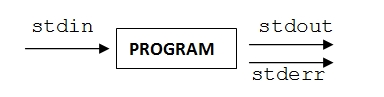
\includegraphics[width=0.5\textwidth]{img/strumienie}
\caption{Strumienie wejście-wyjście}
\label{fig:strumienie}
\end{figure}

Źródło oraz wyjście danych można zmienić stosując tzw. przekierowanie strumieni. Jako strumień wejściowy do programu można wysłać zawartość pliku. Służy do tego zapis:

\begin{lstlisting}[style=MyBashStyle]
# polecenie < plik
\end{lstlisting}


\begin{example}[Przekierowanie strumienia wejściowego]

Polecenie \lstinline[style=MyBashStyle]{cat} wywołane bez żadnych argumentów kopiuje strumień \lstinline[style=MyBashStyle]{stdin} do strumienia \lstinline[style=MyBashStyle]{stdout}. Podaj zawartość pliku \lstinline[style=MyBashStyle]{piszA} jako strumień wejściowy do polecenia \lstinline[style=MyBashStyle]{cat}.

\begin{lstlisting}[style=MyBashStyle]
# cat < piszA
\end{lstlisting}

Strumień wyjściowy \lstinline[style=MyBashStyle]{stdout} możemy przekierować do pliku za pomocą zapisu:

\begin{lstlisting}[style=MyBashStyle]
# cat > mojplik
pierwszy wiersz
drugi wiersz
trzeci wiersz
#                          # Ctrl+C
# cat mojplik
\end{lstlisting}

W ten sposób wyjście z programu zostanie zapisane do pliku \lstinline[style=MyBashStyle]{plik}. Można również sprawić, aby wyjście zostało dopisane do pliku:

\begin{lstlisting}[style=MyBashStyle]
# cat >> mojplik
czwarty wiersz
piaty wiersz
#                          # Ctrl+C
# cat mojplik
\end{lstlisting}
\end{example}


\begin{example}[Przekierowanie strumienia wyjściowego]

Wylistuj zawartość bieżącego katalogu i~przekieruj listing do pliku \lstinline[style=MyBashStyle]{mojplik2}. Wyświetl zawartość pliku \lstinline[style=MyBashStyle]{mojplik2}.


\begin{lstlisting}[style=MyBashStyle]
# ls -la > mojplik2
# cat mojplik2
\end{lstlisting}

Wyjście \lstinline[style=MyBashStyle]{stderr} można przekierować do pliku w następujący sposób:

\begin{lstlisting}[style=MyBashStyle]
# polecenie 2> plikzbledem
# cat plikzbledem
\end{lstlisting}

lub

\begin{lstlisting}[style=MyBashStyle]
# polecenie 2>> plikzbledem
# cat plikzbledem
\end{lstlisting}
\end{example}

\begin{example}[Przekierowanie strumienia stderr]

Próba skopiowania nieistniejącego pliku spowoduje wyświetlenie komunikatu o błędzie. Przekieruj ten komunikat do pliku \lstinline[style=MyBashStyle]{plikzbledem2} po czym wyświetl zawartość pliku

\begin{lstlisting}[style=MyBashStyle]
# cp pliknieist . 2> plikzbledem2
# cat plikzbledem2
\end{lstlisting}
\end{example}

\begin{example}[Jednoczesne przekierowanie strumienia stdin i stdout]
Podaj zawartość pliku \lstinline[style=MyBashStyle]{piszA} na wejście polecenia \lstinline[style=MyBashStyle]{cat} a wyjście przekieruj do pliku wyjscie. Wyświetl zawartość pliku \lstinline[style=MyBashStyle]{wyjscie}.

\begin{lstlisting}[style=MyBashStyle]
# cat < piszA > wyjscie
# cat wyjscie
\end{lstlisting}
\end{example}

\begin{example}[Potoki i~filtrowanie wyników]
Polecenia można łączyć w potoki (ang. pipes). Dokonuje się tego poprzez zapis:

\begin{lstlisting}[style=MyBashStyle]
# polecenie1 | polecenie 2 | ...
\end{lstlisting}

\begin{figure}[!h]
\centering
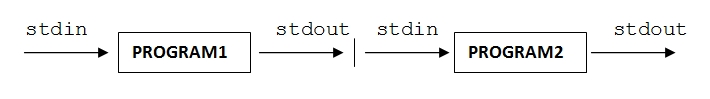
\includegraphics[width=1.0\textwidth]{img/potoki}
\caption{Zasada działania potoków (pipes)}
\label{fig:potoki}
\end{figure}

Wyjście \lstinline[style=MyBashStyle]{stdout} programu1 jest podawane na wejście \lstinline[style=MyBashStyle]{stdin} programu2 itd. Kodem zakończenia potoku jest kod zwrócony przez ostatnie polecenie.

Polecenie \lstinline[style=MyBashStyle]{grep} filtruje przychodzący tekst przepuszczając tylko linie tekstu pasujące do wzorca. Należy "przepompować" zawartość pliku \lstinline[style=MyBashStyle]{piszA} poleceniem \lstinline[style=MyBashStyle]{cat} do polecenia \lstinline[style=MyBashStyle]{grep}, aby wyszukać linie zawierające literę \lstinline[style=MyBashStyle]{A}.

\begin{lstlisting}[style=MyBashStyle]
# cat piszA | grep 'A'
\end{lstlisting}

\end{example}

\begin{example}[Sortowanie i obcinanie wyników]

Wyświetl listę pięciu największych plików w bieżącym katalogu:

\begin{lstlisting}[style=MyBashStyle]
# ls -s | sort -n | tail -5
\end{lstlisting}
\end{example}

\begin{example}[Prosta sekwencja poleceń]

Polecenia można grupować w tzw. sekwencje. Służą do tego operatory \lstinline[style=MyBashStyle]{;}, \lstinline[style=MyBashStyle]{&&} i~\lstinline[style=MyBashStyle]{||}. Polecenia połączone operatorem \lstinline[style=MyBashStyle]{;} wykonują się jedno po drugim bezwarunkowo.

W jednej linii zdefiniuj zmienną o nazwie \lstinline[style=MyBashStyle]{FOO} i~wyświetl jej zawartość.

\begin{lstlisting}[style=MyBashStyle]
# FOO='To jest zmienna FOO';echo $FOO
\end{lstlisting}

\end{example}

\begin{example}[Sekwencja warunkowa - koniunkcja]
Operator \lstinline[style=MyBashStyle]{&&} umożliwia wykonanie następnego polecenia w sekwencji tylko, jeśli poprzednie wykonało się pomyślnie (kod wykonania \lstinline[style=MyBashStyle]{=0}). Polecenie \lstinline[style=MyBashStyle]{grep} zwraca \lstinline[style=MyBashStyle]{0} (sukces), jeśli poszukiwany wzór występuje w tekście. W przeciwnym przypadku zwraca wartość niezerową (błąd). Przeszukać zawartość pliku \lstinline[style=MyBashStyle]{piszA} w poszukiwaniu wzorca \lstinline[style=MyBashStyle]{A} i wyświetlić napis "Znaleziono", jeśli wzorzec wystąpił. Wykonać podobny zabieg dla wzorca \lstinline[style=MyBashStyle]{kawa}.

\begin{lstlisting}[style=MyBashStyle]
# cat piszA | grep 'A' && echo "Znaleziono"
# echo $?
0
# cat piszA | grep 'kawa' && echo "Znaleziono"
# echo $?
1
\end{lstlisting}
\end{example}

\begin{example}[Sekwencja warunkowa - alternatywa]
Powtórzyć poprzedni przykład używając operatora \lstinline[style=MyBashStyle]{||}, zamiast \lstinline[style=MyBashStyle]{&&}.
\begin{lstlisting}[style=MyBashStyle]
# cat piszA | grep 'A' || echo "Znaleziono"
# echo $?
0
# cat piszA | grep 'kawa' || echo "Znaleziono"
# echo $?
0
\end{lstlisting}
\end{example}

\subsection{Ćwiczenia}

\begin{myenumerate}
\item W systemie pomocy znajdź opis programu do archiwizacji danych tar. Spakować wszystkie pliki znajdujące się w katalogu bieżącym (tj. \lstinline[style=MyBashStyle]{/home}) do pojedynczego archiwum o nazwie \lstinline[style=MyBashStyle]{programy.tar} (opcje \lstinline[style=MyBashStyle]{-cvf}). Utworzyć w katalogu domowym, katalog o nazwie \lstinline[style=MyBashStyle]{Dokumenty}. Skopiować archiwum do katalogu \lstinline[style=MyBashStyle]{/home/Dokumenty} i~tam go rozpakować (opcje \lstinline[style=MyBashStyle]{-xvf}).
\end{myenumerate}

\cleardoublepage
